% 来源：OEBPS/Text/Section0001_split_001.xhtml#sigil_toc_id_9

\BookChapter{1}
\section[第1章\q 自己的钱！自己的生活！自己做主！]{第1章\\ 自己的钱！自己的生活！自己做主！}

\begin{BookQuote}
钱做仆人很好，钱做主人很糟。

\hfill ——弗朗西斯·培根爵士
\end{BookQuote}

钱。

钱，这个词能激起人们非常强烈的情感，很少有力量如此强大的词语。

我们很多人甚至拒绝谈钱！我们在餐桌上很忌讳谈论宗教、性、政治，我们在餐桌上也很忌讳谈钱，在工作场合也往往被禁止谈钱。我们或许会在体面的场合谈谈“财富”，但是谈钱太直接了。谈钱这个东西，太俗，太招摇。钱涉及太多个人的东西，而且承载了太多的情感。有钱的人因为有钱感到内疚不安；没钱的人因为没钱而感到羞愧。

但钱对于人们而言到底意味着什么呢？

对于一些人来说，钱至关重要，但它并不是最重要且至高无上的。钱只是一个工具，能够产生力量，用来服务他人，创造更加美好的生活。另外一些人则过分痴迷于金钱，结果毁了自己，也毁了周围的人。有些人为了得到钱，甚至愿意放弃价值更高的东西，比如健康、时间、家庭、自我价值，甚至尊严。

从核心本质来看，钱就是力量。

我们都看到过钱拥有巨大的力量，能够创造，也能够毁灭。钱能够成就梦想，也可以挑起战争。你可以把钱当作礼物送人，也可以把钱作为武器伤人。你可以用钱表达你的精神、创意、想法，也可以用它表达你的沮丧、愤怒和仇恨。钱可以用来影响政府，也可以用来影响个人。有些人真的会为了钱而结婚——后来他们才意识到自己付出的代价有多大。

但我们都知道，在某种程度上，钱只是一种幻觉。现在的钱，早就不是黄金了，甚至连纸币也不是。它只是银行电脑里一连串的零和其他数字的组合而已。钱到底是什么？钱就像变形器，就像画布，你赋予钱什么含义和什么情感，钱就代表什么含义和什么情感。

说到底，钱并不是我们真正想要追求的目的……难道不是吗？我们真正想要追求的是感觉，是情感。我们认为钱可以创造出这些感觉和情感：

权力感，

自由感，

安全感，

助人感——帮助我们爱的人和需要帮助的人，

选择感，

存在感。

把梦想变成现实有很多种方法，钱肯定是其中的一种。

但即使钱只是一种感觉——一种非常抽象的概念，但你如果没有足够多的钱，就感受不到这一点！有件事是可以完全肯定的：要么你用钱，要么钱用你。你要么是钱的主人，要么，至少从某种程度上说，你就是钱的奴隶。

你处理钱的方式可以反映出你对待权力的方式。钱对于你来说是苦恼的还是幸福的呢？赚钱是游戏还是负担呢？

我选择用“钱”做本书的书名时，有些人对赚钱也许只是一种游戏的说法会勃然大怒。对赚钱这样一个严肃的话题，怎么能使用“游戏”这种轻浮且没有重要意义的词语呢？但是，朋友，我们还是面对现实吧。接着读下去，你会明白，改变自己生活的最好方式就是找到那些已经成功达到和你拥有相同目标的成功人士，然后你只需要模仿他们的行为就足够了。想要掌控自己的投资理财吗？找一个投资理财方面的专家，模仿他处理金钱事务的行为方式，你就会踏上发掘金钱力量的成功之路。

现在我可以告诉你，在全世界最有钱的富豪中，我采访过很多人。其中大多数人确实认为赚钱就是一种比赛。否则，为什么会有人已经赚了几十亿美元还要每天工作10个小时甚至12个小时呢？记住，并非所有的游戏都是非常轻浮且没有重要意义的。游戏就是生活的反映。有些人坐在场边当观众；有些人在场上参加游戏比赛，全力争取胜利。你如何参与赚钱这场游戏呢？我想提醒你，赚钱这场游戏，你和你的家人都输不起。

我给你的承诺是：如果你愿意和我一起遵循本书所提出的简单7步投资法——这是我提炼世界上最成功的投资理财高手的经验所总结出来的，你和你的家人就会赢得赚钱这场游戏比赛。你能赚得盆满钵满！

但是要赢得比赛，你就必须知道游戏的比赛规则，向那些成绩好、经验多的高手学习最好的成功策略。

好消息是，你可以节省好几年的时间——只需要花上几分钟——简单地了解需要避开的陷阱和走向永久成功的捷径即可。金融行业里的人在工作中频繁使用专业术语，让人听起来感觉投资理财这件事非常复杂难懂。但实际上，只要你过了专业术语这一关，投资理财这件事相当简单。本书将给你一个翻身做主人的良机，从此让你不再是任人摆布的棋子，而成为金钱游戏中当家做主的棋手。我想你会非常惊讶地看到，自己如何从什么也不懂的外行变成很懂门道的内行，以及很容易就完全改变自己的投资理财计划，从此享受自己应得的财务自由。

让我们一起来努力吧！想象一下，你是技巧熟练、经验丰富的投资理财游戏的比赛高手，你的生活会变成什么样子呢？

如果从此以后钱对于你来说不再重要，生活又会怎么样呢？

原来你天天都要操心的事，每天早上一定要准时上班，账单来了得赶紧支付，养老金要交了。有了钱之后，你再也不用为这些事操心发愁了，你会是什么感觉呢？按自己的意愿，过自己的生活，会是什么样子呢？一旦你知道，自己有机会创立自己的企业，自己有能力给父母买套好房子，自己有财力送孩子上好大学，自己拥有财务自由和时间可以环游世界，你内心会是什么样的感觉呢？

每天早上醒来，你知道自己有足够多的钱，不但能够满足生活的基本需要，而且能实现自己的人生目标和梦想，你会如何生活呢？

事实是很多人还会继续工作，因为我们天生注定要工作。但是有了财务自由之后，我们不再为了钱而工作，而是为了人生更加快乐和生命更加充实而工作。我们的工作会继续下去，但是原来那种为了赚到更多钱的残酷竞争会终止。我们工作是因为我们愿意工作，而不是因为我们必须工作。

这就是财务自由。

这是白日梦吗？对于普通人来说，更重要的是对于你自己来说，这个梦想真的能变成现实吗？

不管你是想赚很多钱，过上令人艳羡的富裕生活，还是只想赚的钱够花就行，事实上，你总可以找到办法赚到足以满足你个人需要的钱。我们该怎么做呢？获得足够多财富的秘诀很简单：找到一条路，让自己能为他人做得更多，比其他人做得都多。让自己变得更有价值。做得更多，给予更多，承担更多，服务更多，你总有机会赚得更多，不管你是在得克萨斯州的奥斯汀拥有最好的快餐车，还是成为公司里的顶尖销售人员，甚至是成为像照片分享应用软件Instagram公司的创始人一样的人物。

但本书要讲的不仅仅是增加价值，实际上本书要讲的是如何实现个人成长，从你现在的低水平成长到你非常想要达到的高水平，无论是财务安全，财务独立，还是财务自由。本书讲的是如何开发一种基本的生活技能，即投资理财能力，以赚到更多的钱，提高你的生活质量，而绝大多数美国人从来没有培养过自己的投资理财技能。事实上，77\%的美国人，也就是4个美国人里就有3个人承认自己为钱发愁，但只有40\%的人揣摩过开支计划或投资计划。美国婴儿潮一代出生的人（1946—1964年出生），3个人里就有1个人存款不足1000美元。民意调查显示，美国民众信任金融体系的比例低于25\%——理由非常充分！持有股票的人数跌到历史低位，在年轻人当中尤其如此。但是，事实上，并不是收入高、赚的多就能实现财务自由。本书后面会讲到，即便收入高达数百万美元的人，如电影《教父》的导演弗朗西斯·福特·科波拉、拳击明星迈克·泰森、演员金·贝辛格，后来也失去了财务自由，因为他们没有运用本书所讲的投资理财的基本原则。你一定要努力为家人保住你赚到的钱，但是更重要的是，你还要让自己赚到的钱能够生钱——你在睡觉的时候也照样赚钱。你必须转变自己，从经济上的财富消费者变成财富所有者。为此你必须成为投资者。

实际上，我们很多人已经是投资者了。你第一次进入投资理财这场游戏比赛，也许是你奶奶为了庆祝你的出生给你买了一些她最喜欢的股票，也许是你的老板自动把你加入公司的401(k)养老金计划，进而开始购买股票基金，也许是朋友告诉你要放下电子书阅读器Kindle去买其生产商亚马逊（Amazon）的股票，从而使你第一次成为股票投资者。

只是这样做就够了吗？你能读到这里，我猜你肯定知道答案是根本不可能。我不用提醒你，现在完全不是你父母和祖父母的投资世界了。过去的人生投资理财计划非常简单：上大学，找工作，努力工作，再跳到更大的公司得到更好的工作岗位；从此以后，投资理财的关键是找到办法为公司增加更多的价值，让自己的职位不断往上爬，投资购买自己公司的股票，拿到一大笔养老金光荣退休。还记得养老金吗？养老金还能保证给你带来持续的收入，永远不会终止吗？这套人生投资理财模式已经落伍了。

我们都知道，时代变了，世界变了。我们的寿命更长，钱却更少了。各种新技术不断涌现，让金融体系更加完善，但设计这个金融体系的目的好像不是帮助我们让自己手里的钱增值更多，而是让我们手里的钱变得更少，跑到别人腰包里的钱更多。当我写下这些文字的时候，美国的存款利率接近0\%，而美国股市像漂在大海上的软木瓶塞一样大起大落。与此同时，我们面临的金融体系给你的选择多到无限大，复杂到你的大脑简直难以想象。如今，美国股市上公募基金\footnote{\label{fn:pdf-1-1}美国人称为“共同基金”，国内称为“公募基金”。——译者注}的数量超过10000种，ETF（交易所交易基金）数量有1400个，还有其他几百个全球各地的股票交易所可供选择。我们似乎每天都淹没在越来越复杂的投资“工具”中，由首字母缩写而成的简称多得让我们眼花缭乱：CDOs（债务抵押债券），REITs（房地产投资信托基金），MBSs（抵押贷款支持债券）……

我们到底该怎么办呢？

HFT怎么样？这是“高频交易”（high-frequency trading）的简称。在证券市场每天几千万次的交易中，50\%\textasciitilde{}70\%是用高速电脑完成的。这对你有什么意义呢？只需半秒钟，大约500毫秒，点击一下鼠标，你就能完成电子交易报单。同样是在短短半秒的时间里，你只买卖一次的股票，使用超级计算机的那些大机构就能买进卖出这只股票好几百次，而且每笔交易都能获得微小的盈利。迈克尔·刘易斯写了一本畅销书《高频交易员》（\textbf{Flash Boys: A Wall Street Revolt}），揭露了高频交易的很多内幕。刘易斯在美国电视访谈节目《60分钟》上说：“美国股票市场，这个全球市场经济体系最有代表性的市场，现在却被联手操纵……操纵者是证券交易所、华尔街大型银行和高频交易员……他们可以预先判断出你想买微软公司的股票，然后可以在你之前抢先买入，再转手用更高的价格卖给你！”这些高频交易员的交易速度到底有多快呢？一家高频交易公司花费2.5亿美元改造芝加哥和纽约之间的光缆，让其变得更直、更短，而且重整光缆周围的地形地貌，结果让芝加哥和纽约两地之间的数据传输时间减少了1.4毫秒！但这么快还不够。有些交易完成的时间只需几微秒——1微秒等于1/1000000秒。不久，高频交易技术就能把交易完成时间缩短到纳秒，也就是1/1000000000秒。与此同时，他们正在海底铺设电缆，他们甚至要用太阳能无人机作为微波中继站，来连接纽约和伦敦的证券交易所。

如果我前面讲的这些投资新时代下的新世界的复杂情况，让你感到头昏脑涨，别担心，我会陪着你。和光速一般高频交易的机器人在证券市场上竞争，你的胜算有多大呢？在证券市场这个选择多得无法计算而且充满高科技、高风险的迷宫里，你如何找到一条成功之路顺利地走出迷宫呢？

\begin{BookQuote}
专家就是走出家门给人提供建议的普通人。

\hfill ——奥斯卡·王尔德
\end{BookQuote}

问题是一谈到钱（和投资），每个人都有自己的看法，每个人都有自己的贴士，每个人都有自己的答案。但我要给你一个提醒：极少有人能真的帮到你。你注意到了人的金钱观与宗教观、政治观有多么相似吗？谈起钱，就像谈起宗教和政治一样，人会变得言辞激烈，情绪激动。尤其是上网聊天的时候，即便自己没有真才实学，也没有操作经验，你照样会极力宣扬自己的理论，激烈地批评他人的策略。其实，这就像一个心理学家患上抑郁症，自己也治不了自己，只能偷偷吃百忧解，却天天教导别人如何走出抑郁，过上幸福美满的生活。或者说这就像自己是个超级大胖子，却滔滔不绝地讲述如何减肥保持身材。我一般会把专家分为两类，一类专家是光会说不会干型，另一类专家是自己会干也会教你干型。我不知道你喜欢哪一类，但是我很厌恶那些光会说不会干的“伪专家”，滔滔不绝地告诉别人这么干效果会有多么好，但是自己在生活中干得一点儿也不好。

如果你觉得读本书又会让自己听到一个投资大师吹嘘自己，兜售自己，发疯一样地承诺跟着我做肯定大赚，我想你找错地方了。那种事情，还是留给那些金融行业里的表演大师去做吧。这些金融行业里的表演大师会高喊快去买哪个热门股，诱导你攒一笔钱去投资那些神话般的公募基金。你知道的，他们承诺，你投入的钱将会以每年12\%的复利收益率持续增长。这些所谓的投资理财专家随随便便提出的建议根本不现实，而且他们自己都不投资自己推销的产品。其中有些投资理财专家也许认为自己是在真心实意地帮助别人，但是你知道很多人真心实意地帮忙，反而是真心实意地帮了倒忙。

我想让你知道，我并不是一个“积极思考者”，用错误的世界观来激励你、推动你。我相信的不是激情，而是头脑。你要看到事物的真实面目，但不能过度乐观，同时也不能过度悲观。因为这样的世界观只会让你找到什么也不做的借口。你可能在电视上看到过我，就是“那个微笑着露出大牙的家伙”，但我在这里要告诉你的并不是做一堆自我肯定来提高自信——我一直努力专注做的事情是，帮助你深入认识自我，解决实际问题，提升自己的人生以达到更高的层次。

38年来，我一直痴迷于寻找各种策略和工具来立即改变人的生活品质。我用事实证明，用别人的方法都失败了。但是同样的问题，用我的方法却成功了，效果既看得见，又摸得着，更算得清。我的课程影响力越来越大，到目前为止，100多个国家中的5000多万人购买了我的书、视频和音频课程，超过400万人参加了我的现场活动。

我从一开始就知道，成功有迹可循。成功达到最高水平的人并不只是因为幸运而已，而是因为他们有些事的做法与众不同。我感兴趣的是这样的成功者：坚持不懈地渴望学习、成长和获得成就。别误会我的意思，我不会轻易地受人哄骗。我很清楚，世界上少有人能永远身体健康。大多数人都无法做到几十年如一日地在亲密关系中持续保持热爱与激情，也无法做到几十年如一日地持续感到感激和快乐。只有极少数人能抓住商业机会并做到极致，更少的人能够白手起家实现财务自由。

但是确实有少数人做到了！这些少数派确实拥有极好的亲密关系、极大的快乐、超级多财富和无尽的感激之情。我研究对比过少数实干者和多数空谈者。如果你要找的是障碍，做错的行为到处都是。但是，反过来也如此，你要找的是捷径，做对的行为也比比皆是。我要找的目标是卓越的成功人士。我要找的是那些打破常规不走寻常路的创新成功者，他们向我们所有人展示出一切皆有可能。我学习了解了少数特别成功的人的与众不同的做事方法，然后全力模仿他们。我从模仿实践中找出哪些方法确实有效，然后明确描述出来，简化概括出来，系统总结出来，然后利用它们去帮助其他人发展、进步、提高。

2008年，在那些黑暗的日子里，全球金融体系几乎完全崩溃。从此以后，我每天都痴迷于找到一种投资理财之道，帮助人们掌控自己的金钱，以反击现在经常受到操纵、巧取豪夺民众财富的美国金融体制。在金融危机之后，修补金融体制的工作已经持续进行了很多年，但所谓的“国会山改革”并没有实现金融体制整体的变革，美国金融体制有些方面反而变得更糟糕了。为了找到正确的投资理财之道，我采访了全球金融界最出色也最有影响力的投资理财高手。本书不会讲空话大话，也不会讲我个人的观点。你能直接听到来自投资理财大师本人的原汁原味的建议。他们是自己打拼出来的亿万富翁、诺贝尔奖得主、金融大亨。后面我们会详细介绍很多投资理财大师的观点，供大家参考学习。先简单列举几位投资理财大师：

\begin{itemize}
\item 约翰·博格，现年85岁的“指数基金之父”，64年股市投资经验，世界上资产规模最大的公募基金公司美国先锋公司的创始人。
\item 瑞·达利欧，全球规模最大的对冲基金创始人，管理资产规模高达1600亿美元。
\item 戴维·斯文森，有史以来最伟大的机构投资者之一，只用了不到20年，就把耶鲁大学的捐赠基金从10亿美元增长到239亿美元以上。
\item 凯尔·巴斯，在次贷危机期间，只用2年时间，就将3000万美元投资增值到20亿美元。
\item 卡尔·伊坎，最近1年、5年、10年的投资业绩跑赢沃伦·巴菲特，跑赢股市，可以说跑赢所有投资人。
\item 玛丽·卡拉汉·厄道斯，许多人认为她是金融界最有权势的女人，她担任摩根大通资产管理公司的首席执行官，管理资产规模超过2.5万亿美元。
\item 查尔斯·施瓦布，领导发起证券行业革命，让华尔街证券机构向个人投资者开放，嘉信理财公司现在管理资产规模达2.38万亿美元。
\end{itemize}

现在阅读本书，你就能与50位超级投资明星大师共聚一堂。我要引见给你的还有其他的投资大师，无论市场是涨是跌，经济是繁荣还是衰退，这些投资超级明星都是十年如一日地持续获得良好的投资业绩。我们一起来揭开他们投资成功的核心秘诀，看看如何将这些秘诀运用到我们的、哪怕是规模最小的个人投资上。

其中的关键是，本书的根基是50位世界上最成功的投资理财大师永恒的投资智慧。毕竟，所有阅读本书的投资者，没有一个人能够预测到未来宏观经济的走势。货币会是通货膨胀还是通货紧缩？股市会是牛市还是熊市？你应该知道的是，不管遇到任何市场情况，我们都能生存下来并且发展壮大。这些真正的专家会告诉你如何做到这一点。另外，他们会打开自己的实际投资组合，展示给你他们是如何通过混合搭配不同种类和数量的证券而安然渡过了一次又一次市场风暴的。他们还会回答这个问题：如果你一点金融财富也不能留给孩子，只能留给孩子一套投资法则，那么这套法则会是什么呢？这可能是投资大师最宝贵的遗产。你不用是他们的孩子，也能得到大师的真传。

\begin{BookQuote}
领先的秘诀就是尽快开始。

\hfill ——马克·吐温
\end{BookQuote}

准备好，因为我们即将一起开始简单7步投资法之旅，走向财务安全、财务独立、财务自由。无论你是千禧一代（1984—2000年出生的人），1946—1964年婴儿潮时代出生的、现在面临退休的老年人，是希望保持领先优势的资深投资者，本书都会为你提供一份实际的蓝图，帮你制定并实现财务目标，帮你摆脱那些自我限制的行为，避开可能阻碍你获得足够财富、实现财务自由的障碍。我们会探索关于财富的心理学，其中有些财富心理学知识，我已经研究并讲授了近40年。我们将纠正人们在处理钱的问题上所犯的错误，像重新校准枪械一样，回归最妥善的计划，稳步前行。为了保证你能得到自己想要的结果，我向世界上最好的行为经济学家取经，寻找真正有效的行为矫正的解决办法——只需要做一些很小而且很简单的调整，就能自动触发你做到别人需要很严格的纪律约束，而且持续坚持才能做到的事情；教你采取一些有效的投资策略，让你赚到的财富足以使你享受舒适的晚年退休生活，而不是亏个精光，无奈破产，在贫困潦倒中死去。

\begin{figure}[htbp]
\centering
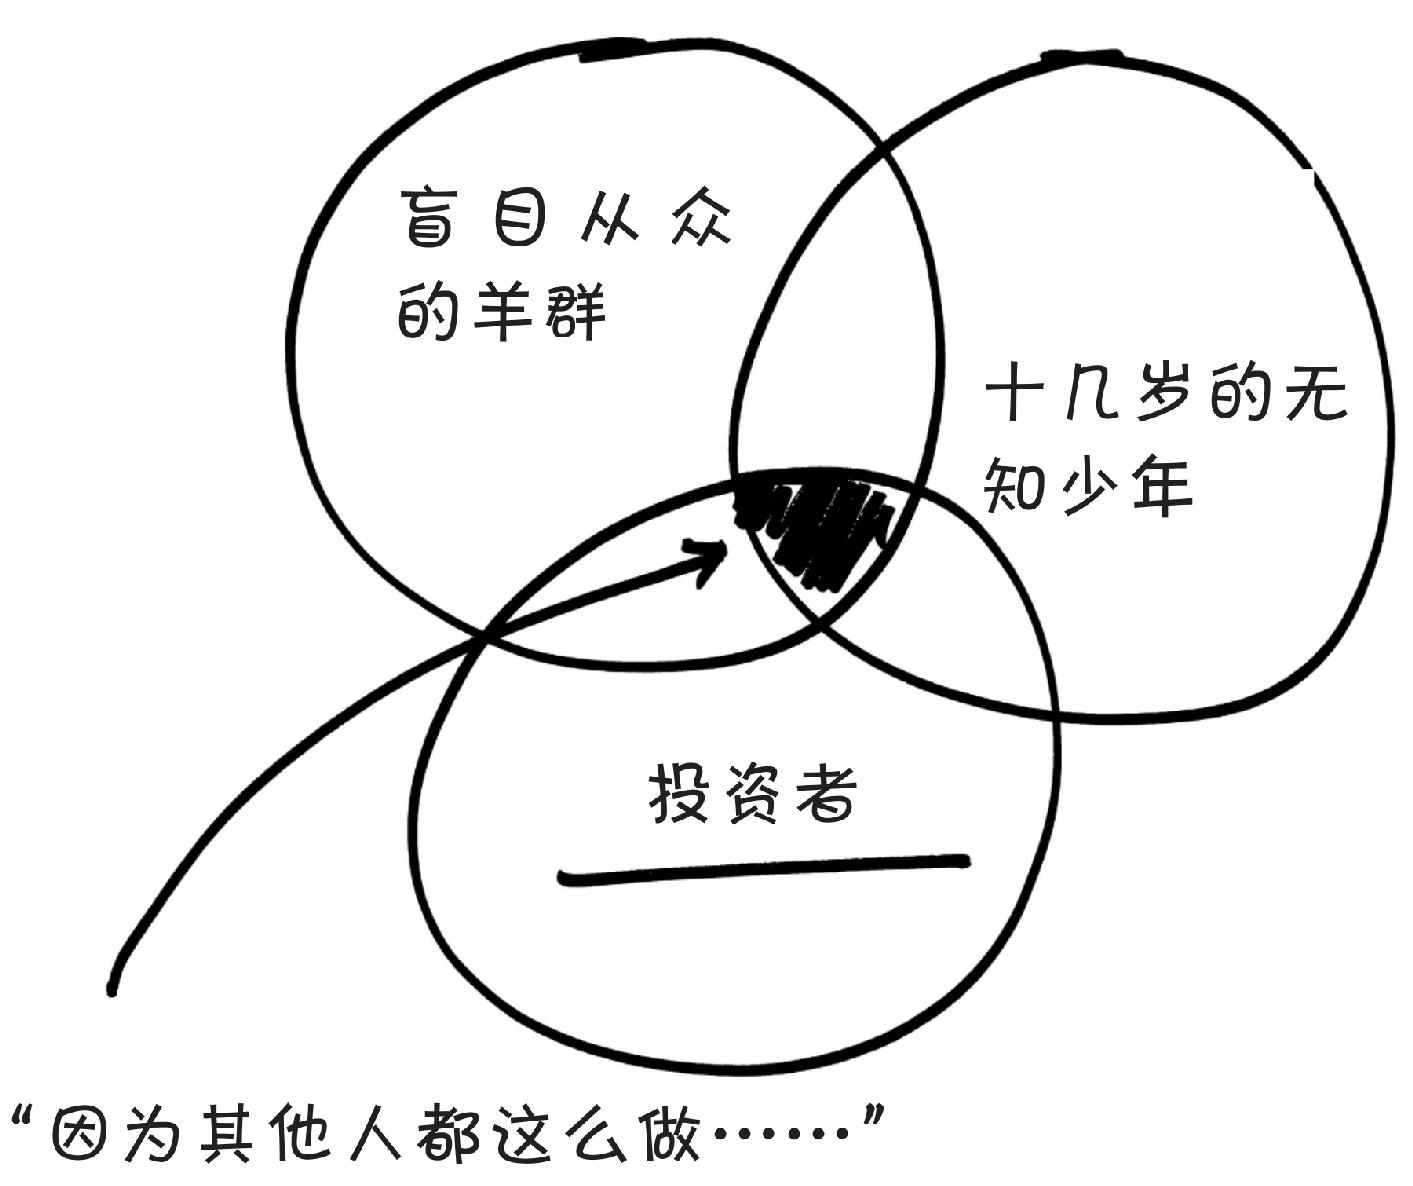
\includegraphics[width=0.68\linewidth,keepaspectratio]{image/1-1.jpg}
\caption{}\label{fig:1-1}
\end{figure}

我们要直面现实：很多很聪明、很有成就的人一碰到钱的事情就选择逃避，因为钱的事情看起来太复杂了。我邀请的第一批审阅本书初稿的人中，有位名叫安吉拉的朋友，她在许多方面都很有成就，但在钱的事情上却很失败。安吉拉告诉我，大家都觉得她很了不起，是因为她驾着一只小小的帆船，在世界上最凶险的海域上，独自一人航行了20000英里\footnote{\label{fn:pdf-1-2}1英里≈1.61千米。——编者注}。但她清楚地知道，自己完全不打理自己的财务，因为投资理财这件事让她很头疼。安吉拉坦诚地告诉我：“投资理财看起来很复杂，我感到很困惑，我觉得自己根本没有能力做好投资理财。我曾经在投资理财上犯过错误，很受打击，所以我就放弃了，虽然这非常不符合我的性格。”但她读了本书的初稿之后便发现，只要按照书中简单7步投资法去做，她就能够掌控自己的投资理财事务。这7个步骤很容易做，而且没有任何痛苦！她告诉我：“我的天哪，我竟然也能存些钱，应对未来了。只要放弃购买那些不能给我带来快乐的东西就行了。”一旦开始考虑存钱，她就能开立一个自动投资账户。当读到本书的第13章时，她在投资理财上做出的认识变化，已经改变了她的人生。

几天后，她专门来看我，高兴地说：“我这辈子第一次买了一辆崭新的汽车。”

我问她：“你是怎么做到的呢？”

她回答：“我读了你写的书才开始意识到，我原来开的旧车平时花的修车费和油费太高了，比贷款买辆新车的月供还要高！”她开着一辆白色的吉普牧马人，崭新崭新的，简直光芒四射。你可以想象到她的笑容是何等的光辉灿烂。

所以我想让你知道，本书要讲的不仅是如何拥有舒适的退休生活，而且是如何拥有你想要的，也本应该是今天就拥有的高品质生活。你能过上自己想要的那种生活，同时可以确保未来能继续保持同样高品质的生活！掌控了钱的事，会让你对外充满权力感，向内充满力量感，决策充满确定感。这些美好的掌控感会传递到你生活的其他方面——掌控你的职业，掌控你的健康，掌控你的情绪，掌控你的人际关系。无法掌控自己的钱，对自己的投资理财能力缺乏信心，这会在不知不觉中影响你在其他方面的自信。当可以完全掌控自己的财务状况时，你就会赋予自己力量，激励自己勇于接受其他方面的挑战！

是什么因素阻碍了我们开始走上财务自由之路呢？对于我们很多人来说，比如我的朋友安吉拉，只是心里那种感觉阻碍了我们前行。一直有人灌输给我们这样的想法：“投资理财这事太复杂啦。”“这事我不内行。”坦白来说，那些专业人士故意把金融体制设计得让人觉得复杂难懂，因为这样你就会干脆放弃属于自己的掌控权，把它全部交给“专业人士”。他们却完全把你蒙在鼓里，让你一无所知，这样你就会心甘情愿地付给他们很高的手续费。阅读完后面的几章，你能学会如何防止这样的事情发生在你头上，最重要的是，我会展示给你看，用你自己的方式来掌握投资理财，最终实现财务自由。其实这样的操作一点儿也不难。

人能成功的原因之一是知道别人不知道的知识。你花钱请律师打官司，花钱请医生看病，是因为他们有你所没有的知识和能力。专业人士也有自己的专业术语，这些术语我们这些外行根本听不懂，所以有时我们会感觉隔行如隔山。

例如在医学界，你可能会听到在过去的一年里有225000人的死亡属于“医源性死亡”。根据《美国医学协会杂志》的报道，这是美国的第三大死因。医源性死亡是什么意思？这个术语听起来很重要，但到底是什么意思呢？这是一种罕见的热带疾病，还是基因突变呢？都不是。医源性死亡实际上指的是，医生、医院不正确或不必要的医疗程序所导致的意外死亡。

他们为什么不用这样的大白话来讲呢？因为用外行都能懂的话来说，不符合医疗机构的利益。金融界也有自己的行话，那些专业术语描述的东西，其实都是额外多收的手续费。有了这样听起来令人费解的语言做伪装，就能故意让那些外行客户听不懂，好让你完全意识不到金融机构收取的手续费，比你能想象到的最高水平还要多得多。

我希望你能让我做你的翻译，同时担任这次通向财务自由之旅的向导。因为正是那些复杂难懂的专业术语，让我们觉得自己是金融界的外行，不找内行的专业人士帮助根本行不通。我带你一起破译这些像密码一样的金融专业术语，让你这个外行也一样能听懂那些金融专业人士的行话。

现在这个时代的信息太多了，即使最有经验的投资者也会感到信息过载，特别是当我们意识到自己接收的信息往往与自己的需求无关时。例如，你胸口有轻度疼痛，于是你用谷歌搜索“心”这个字。你会得到什么样的搜索结果呢？你搜索到的结果，并不是那些你现在想要处理的有关心脏病的信息，而是一个叫作“心”的乐队组合，尽管他们唱了20年也没红过。这种搜索结果对你有什么用呢？

我的计划是为你提供服务，成为你的个人投资理财搜索引擎——智能搜索引擎，帮你过滤掉多余的甚至是有害的金融信息，提供给你简单明确的解决方法。

不知不觉地，你也成了内行。你会明白为什么追逐高业绩明星基金这一招从来不会灵，为什么没有人能长期战胜市场\footnote{\label{fn:pdf-1-3}除了少数几个“独角兽”，也就是人数很少而且限制严格、难以加入的“金融奇才”团队，普通大众根本没有机会接触到，但我会在后面几章中为你介绍。}，为什么绝大多数金融专家没有要为客户利益最大化服务的法律责任。这太不可思议了，对吧？你会明白为什么公募基金在广告中说的基金业绩，并不是你买了基金后真正能到手的业绩。我在本书里讲的投资理财之道，可能会让你一生的投资收益增加几百万美元——统计研究表明，仅仅是阅读和运用本书第二部分所说的投资理财的基本原则，就能为你节省15万\textasciitilde{}45万美元！你能把钱装回到自己的口袋里，而不是装到那些炮制出种种手续费的金融机构的口袋里。你还会学习掌握一条被事实证明了的行之有效的投资理财之路，它让你的钱能够持续增值，而且100\%保本，投资收益免税（由美国国税局批准）。这种投资理财工具终于也向你这样的个人投资者开放了。

这正是本书真正与众不同的地方：我并不是仅仅告诉你那些超级富豪用的是哪些投资策略，这些策略你根本负担不起或者根本没有机会使用。我还找到了解决办法，让那些投资策略普通工薪阶层也能负担得起，也有机会享受得到。凭什么只有那些特权阶层的人才能搭上非同寻常的投资机会呢？现在是不是到了我们可以和超级富豪在投资理财的赛场上公平竞争的时候了呢？

记住，这是你的钱，是时候自己掌控自己的钱了。

\begin{BookQuote}
瞬间的领悟有时候值得用一辈子去体验。

\hfill ——奥利弗·温德尔·霍姆斯
\end{BookQuote}

在开始之前，我要告诉你是什么事触动了我写这本书。如果这些年你看过一些关于我工作的报道，或者你读过我以前写的书，你可能会知道由我创造出来的、可以被衡量的巨大变化纪录——帮助肥胖者成功减重30\textasciitilde{}300磅\footnote{\label{fn:pdf-1-4}1磅≈0.45千克。——编者注}，帮助夫妻彻底扭转即将结束的亲密关系，帮助企业老板一年之内提高30\%\textasciitilde{}130\%的业绩。我还帮人们战胜了巨大的灾难打击，从失去孩子的夫妇，到阿富汗战场归来患上创伤后应激障碍的士兵，让他们重新面对人生。我充满激情的强烈爱好是，帮助人们实现真正的突破性进展，包括人际关系、情绪、健康、事业、理财五大方面。

近40年来，我有幸担任教练帮助各行各业的人提升自我，其中包括这个世界上最有权势的男人和女人。我训练指导过的人，既有美国的总统，也有小企业的总裁。我作为教练，训练和帮助过体育明星提高成绩，从早期合作过的冰球巨星韦恩·葛雷茨基到现在合作的网坛巨星小威廉姆斯。我也有幸与多位荣获大奖的明星演员合作过，他们既有冷酷似冰的莱昂纳多·迪卡普里奥，也有热情似火的休·杰克曼。我的工作能接触到顶尖艺人的生活和演出，从史密斯飞船乐队到绿日乐队，从厄舍到皮普保罗，再到小埃勒·库尔。我也指导过拥有亿万财富的企业领袖，如赌场巨头史蒂夫·韦恩和互联网“鬼才”马克·贝尼奥夫。事实上，正是在1999年参加了我的一场名为“释放你的内在力量”的研讨会之后，贝尼奥夫才下决心从甲骨文公司辞职，开始创建Salesforce.com公司的。今天，Salesforce.com公司价值50亿美元，连续4年获得《福布斯》“全球最佳创新企业”称号。很显然，客户找我不是为了寻求激励，他们已经有足够多的激励了。客户从我这里得到的是策略，以帮助自己提升到更高层次，持续保持顶尖的竞争地位。

在金融领域，我很荣幸，从1993年以来，一直在指导保罗·都铎·琼斯，他可以称得上是有史以来十位顶级投资大师之一。保罗成功地预测了1987年10月黑色星期一的美国股市大崩盘——迄今为止，仍然保持美国股市最大单日跌幅的历史纪录（按百分比算）。虽然全球股市暴跌，所有人都亏得连短裤也输掉了，保罗却在1987年赚了整整1倍。2008年，保罗再造神话，整个美国股市暴跌50\%，他却赢利近30\%。我和保罗合作要做的事情就是，捕捉到那些引导所有投资决定的基本原则，然后把这些基本原则综合成一套体系，让他能够天天使用，最重要的是，在关键的时候他也会运用。我不是一个指导积极思考的人生教练。相反，我是一个训练指导你做好一切准备的人生教练。我和保罗一直保持着联系，并持续追踪他每天的交易情况，一起经历跌宕起伏的各种各样的市场行情。从20世纪90年代后期的科技股泡沫到“9·11”恐怖袭击事件重创股市，我一直和保罗在一起。从房地产大繁荣到次贷危机，再到2008年金融危机，再到后来的欧洲债务危机，再到2013年金价创下30年来最大单日跌幅，我一直都在追踪保罗的交易，我一直和保罗在一起。

尽管经历了以上如此多的巨大困难，在过去连续28个完整年度里，保罗从来没有一年亏损过。这28年里，我和保罗合作了21年。他寻找胜利之路的能力是无与伦比的。无论市场如何波动，保罗总是能持续赚钱，我很荣幸能有机会和他并肩战斗。通过和保罗合作，我更深入地了解到，投资世界的现实情况是什么，在困难时期应该如何制定决策。这比我去读MBA（工商管理硕士）的100门课程所学到的还要多。

同样非常幸运的是，在此期间，保罗不仅在工作上成为我紧密的合作伙伴，而且在生活中保罗也成为我最亲密的朋友之一。我非常热爱保罗，也非常敬重保罗，因为他不仅是全世界业绩最优异的投资人之一，也是全世界贡献最巨大的慈善家之一。多年来，我亲眼见证了保罗领导罗宾汉基金会不断发展壮大。罗宾汉基金会最初只想运用自由市场的力量来减轻纽约市的贫困问题，如今它已经发展为被《财富》杂志盛赞为“最创新又最有影响力的慈善组织”之一。罗宾汉基金会至今累计捐赠了14.5亿美元，改变了几百万人的生活。

一路走来，我也从个人经历中学到了一些教训，有些教训是经历痛苦折磨和错误打击才能学到的——我写本书的意图就是要帮你尽量避免这些错误。我不是空口乱说，我身上还有证券市场给我的重大打击所留下的伤疤。我领导一家股份公司在交易所成功上市，当年我只有39岁，年轻有为，亲眼看到公司股价大涨，短短几个星期，我的个人财富就飙升到4亿美元以上。后来，2000年网络股泡沫破裂，我的公司股票暴跌，个人财富也大幅缩水。

但那时的股市回调，与我们最近几年的金融危机相比，根本不算什么。2008—2009年的金融危机是美国“大萧条”以来最严重的经济危机。你还记得当时整个金融世界好像末日降临一般的感觉吗？道琼斯工业指数暴跌50\%，让你的401(k)养老金投资账户的资产也缩水一半。房价跌了个底朝天，你自己家住的房子的房价随之下降四成，甚至更多。数百万人一生辛勤工作所赚的钱都亏掉了，还有数百万人连工作也丢掉了。在非常恐怖的那几个月里，我接到了各种各样的人打来的求助电话，比以往任何时候都要多。理发师向我求助，亿万富翁也来向我求助。人们告诉我，他们亏掉了房子，他们亏光了储蓄，他们的孩子都没钱上大学了。听到这些，我非常难受，因为我也有过亲身体验。

我一直努力工作，很幸运财务状况良好，比较富裕，但是我并不是从小就是这样的。我在加利福尼亚州沙尘飞扬的圣盖博山谷长大，有过4位不同的父亲。我现在还清清楚楚地记得，那时我还是个小孩子，不用拿起电话，也不用应声开门，我就知道门外的人是谁——讨债的人，但我们根本没钱还债。年少时，我不得不天天穿旧校服上学，那是从旧货店花0.25美元买来的，我感到很难为情。你要是穿得不时尚，别的孩子真的会非常“残酷”地对待你。现在，去旧货店买旧货穿却成了时尚的标志——我真想不到！后来，我终于有钱买人生的第一辆汽车了，那是一辆破旧的1960年款大众甲壳虫，但是那辆旧车没有倒车挡，所以我只能把车停在一座小山上，而且我从来没有足够的钱去买汽油。感谢上天，我从不认命，从不相信“生活就是这样”的那一套说法。我找到了方法来战胜困境。因为我有亲身体验，所以每当我看到有人经受苦难就会受不了。这简直让我急得发狂。2008年给美国人带来的本来可以避免的巨大经济磨难，比我至今所见到的还要多得多。

股市大崩盘发生后不久，每个人都一致同意，必须采取一些措施来完善整个金融体系。我一直在等待这些政府承诺的改变真正发生，但过了几年之后，还是一切照旧。我了解金融危机的根源越多，就越生气。后来我的愤怒爆发了，引爆点就是奥斯卡金像奖获奖纪录片《监守自盗》（\textbf{Inside Job}）。纪录片主演是马特·达蒙，讲的是那些华尔街大作手用客户的钱进行投机，其风险巨大到几近疯狂，几乎颠覆整个美国经济。这些罪犯受到了什么样的惩罚呢？我们这些纳税人出钱把他们救了出来，而且差不多还是让这一帮人来负责经济复苏。看到影片结尾，我气得咬牙切齿，无比愤怒，但是我“化愤怒为问题”：我能做些什么呢？

答案就是写这本书。

\begin{BookQuote}
书是最忠诚的朋友。

\hfill ——欧内斯特·海明威
\end{BookQuote}

做这样的决定可不容易。我都快20年没有写一本大书了。上一年，我平均每隔四天就要乘飞机出差一次，去过的国家超过15个。我管理着十几家公司，还管理着一家非营利组织。我有4个孩子，1个了不起的妻子，还有一个我无比热爱、赖以为生的人生使命。要说我的人生非常充实，一点儿都不为过。我写的《激发心灵潜力》和《唤醒心中的巨人》都是全球畅销书，受到读者热烈的欢迎。但直到现在，我从来没有感受到再次动笔写书的动力。为什么？因为我更爱举办现场活动，我很喜欢那种完全沉浸式的体验，同时与5000人甚至10000人一起交流，即时、灵活地沟通，让他们周末两天持续集中注意力长达50个小时。现在这个时代，就算观看斥资3亿美元拍摄的电影，大多数人都无法坚持坐上3个小时。我清清楚楚地记得，奥普拉告诉我她根本不可能待上2个小时，但是12个小时之后，她站在椅子上，对着镜头大喊：“这是我一生中最棒的体验！”厄舍告诉我，他喜爱我举办的现场活动，但肯定无法坚持听上整整一个周末。就像奥普拉一样，最终，这两天成了他一生中最快乐的体验。50个小时之后，他对我说：“这就像我听了一场人生中最棒的音乐会！我发疯似的记笔记，你让我笑得前仰后合！”

参加我举办的现场讲座活动，会让你的体验充满情感、音乐、激动，以及深刻的洞见，激励你采取重大的行动。参加者不仅思考、感受，而且会改变行为，就像换了个人一样。我的肢体语言，我的声音，是我教学风格的关键。所以，我必须承认，当我坐下来写作的时候，我感觉有块东西堵住了我的嘴不让我说，有人把我的手绑到了后背上不让我写！而且，我发现做一场TED演讲（美国一家非营利性会议机构，以技术、娱乐和设计为主旨举办的演讲活动），就可以影响到上千万名观众。所以，我还有什么必要写书呢？

又是什么让我改变了主意呢？

金融危机造成了巨大的痛苦，但它也让我们重新评估什么才是我们生命中最重要的东西——生命中最重要的东西与钱无关。是时候了，我们要回到本源，回到支撑我们度过困难时期的价值观了。我目睹了金融危机的巨大灾难，这让我想起了自己过去的日子，睡在车上无家可归，却在执着地寻找改变人生的方法。那时是什么改变了我的人生呢？书！是书籍帮助我重塑自我。我一直是一个贪婪的阅读者。年轻的时候，我下决心要一天读一本书。我认为领导者就是阅读者。我上了一门速读课。我确实没有做到一天读一本书，但是过了7年多，我读的书超过了700本。我想从书中找到答案来帮助自己，也帮助他人。我读书的范围很广，心理学、时间管理、历史、哲学、生理学，都有涉猎。我想知道所有可能立刻改变我的人生和别人人生的东西。

但是，小时候我读过的书给我留下的印象最深刻。这些书引领我走出了痛苦的世界——一个没有迷人未来的世界。这些书把我送到了一个拥有无限可能性的新王国。我还记得其中有一本书是拉尔夫·瓦尔多·爱默生写的，里面有一篇论自力更生的文章，其中有几句是这样说的：“每个人的自我教育中都会经历这样一个时期，他终于意识到忌妒即无知，模仿乃自杀。每个人都必须接受自我，无论是好还是坏。”另一本书是哲学家詹姆斯·艾伦写的《做你想做的人》，书名与《圣经》中那句箴言遥相呼应：“因为他心怎样思量，他为人就是怎样。”我读到这本书的时候，恰好内心充满恐惧，正在激烈斗争。詹姆斯·艾伦教导我，我们人生创造的一切都源于思想。

我如饥似渴地阅读伟人的传记，包括伟大的领导人、伟大的思想家、伟大的实干家，比如亚伯拉罕·林肯、安德鲁·卡内基、约翰·肯尼迪、维克多·弗兰克。我认识到，世界上的伟人经历过的痛苦与折磨程度远远超过我。这些伟人能够成大事，并不仅仅因为幸运或者有福气，更多的是因为他们心中有某种东西——一种无形的力量，让他们不能只满足于现状，而要追求发挥所有潜力，做到极致，成为极致，付出到极致。我认识到人生经历并非命中注定，我的过去并不等于我的未来。

另一本我特别喜欢的书是1937年以来美国最经典的成功学名著，拿破仑·希尔的《思考致富》。20世纪初，希尔花了20年时间，采访了当时世界上500位最有成就的人，包括安德鲁·卡内基、亨利·福特、西奥多·罗斯福、托马斯·爱迪生，想要找出这些人成功的共同秘密。希尔发现，这500个成功人士都有一个共同特点——坚持不懈地长期专注于自己的目标，融汇强烈的愿望、坚定的信仰、持久的耐心于一身，不断地努力去实现目标。希尔告诉我们，普通人也可以克服一切障碍，并取得成功，这给那一代在大萧条时期挣扎的读者带来了希望。这也让《思考致富》成了美国有史以来最畅销的书籍之一。

拿破仑·希尔的《思考致富》一直是我的榜样。仿照他的这本经典名著，本书也系统地总结了世界上50位投资精英中的精英的投资成功之道，从沃伦·巴菲特到理查·布兰森爵士，还包括业内专家称之为“当代爱迪生”的科学家雷·库兹韦尔。他发明了第一个数字音乐合成器，而且发明了第一个将文本转换成语音的软件。雷·库兹韦尔就是苹果公司iPhone手机语音助手Siri背后的男人。他还发明了一种设备，能够让盲人安全地过马路，读路标指示牌上的文字，顺利地从任何菜单中点菜。如今，雷是谷歌公司的工程研发主管。但是我要写的这本书，超越了心理学和成功学那些浅层心理层面的东西，会为你提供实实在在的计划，实实在在的工具，让你用它来为自己和家人建设一个更加美好的未来。本书会是一本手册、一个蓝图、一份新经济时代的实用指南。

当我开始重新关注书的力量时，我想：“我需要把解决这些投资理财问题的答案，用一种人人都可以获得的方式传播出去。”借助当今的科学技术，可以为本书带来两大优势，以更好地推动你前行。第一个优势是，本书有些部分提供了电子版，你可以上网观看我对一些投资大师的采访视频。第二个优势是，我们还专门设计开发了一个手机App（应用程序），用来激发你走完这7个简单的步骤，因此你学习的不只是理念，还可以跟着手机App的指导实际操作，让你实现真正与你的潜力相符的财务自由。

顺便说一下，我一开始写这本投资理财书的时候，很多人都说我这是在冒险，肯定是疯了。很多所谓的专家，甚至是朋友警告我，想把非常复杂的金融专业知识传授给普通读者，只有傻瓜才会做出这样的傻事，甚至我的出版商都恳求我还是写些别的东西好了。

但我知道，我能做到。只要我找到最优秀的投资大师来做指导，我就一定能完成。我这里采访到的投资大师，大多数人从来都不接受采访，即使有人接受过采访，也极其少见。尽管这些投资大师也曾在瑞士达沃斯的世界经济论坛上演讲过，或者曾在美国外交关系委员会演讲过，但是把自己的知识讲给普通大众，而且是用普通大众能够听得懂的大白话来讲，这种事他们从来没有做过。用简单易懂的方式，分享投资大师的关键观点，让任何一个人都可以照着去做，成了本书的核心任务。

我很荣幸能和一些世界上最有影响力的人保持良好的关系：地位很高的朋友愿意为了我而打几个电话找人帮忙。很快，我发现大门向我敞开了，我接触到了这些投资理财游戏中的赚钱高手。

\begin{BookQuote}
欢迎来到丛林……

\hfill ——枪炮玫瑰乐队《欢迎来到丛林》
\end{BookQuote}

那么从哪里开始呢？我决定从一个大多数人从来没有听说过的人开始，尽管他被称为“投资界的史蒂夫·乔布斯”。你问任何一位全球金融界的领袖人物，无论是美国联邦储备系统（美联储）的主席、投资银行的负责人，还是美国总统，他们都知道瑞·达利欧。每个金融界的头面人物都会阅读瑞·达利欧每周所写的投资简报。为什么？因为政府机构要打电话咨询他应该如何投资，政府要把钱交给他来投资，养老基金和保险公司也一样。瑞·达利欧是桥水基金的创始人。桥水基金现在是世界上管理资产规模最大的对冲基金，目前资产管理规模有1600亿美元，而一般的大型对冲基金的资产管理规模平均只有150亿美元。想要成为桥水基金的客户，你需要有50亿美元的净资产，初始投资额1亿美元起。但是你现在不用想了，瑞·达利欧根本不会管理你的钱——谁的钱他都不管。

调查瑞·达利欧的出身背景，你会发现他好像根本不可能成为投资专家。他出生于纽约市皇后区，父亲是个爵士音乐家，母亲是个家庭主妇。瑞·达利欧最开始的工作是做球童，在当地的高尔夫课程上第一次接触到股票。如今，瑞·达利欧的个人财富达到140亿美元，在全美富豪排行榜上名列第31位。他是如何白手起家，通过投资成为超级富豪的呢？我一定要搞清楚！这家伙的投资业绩真了不起，根据《巴伦周刊》的报道，他管理的纯阿尔法基金，过去20年里只有3年亏损，2010年他为核心客户创造了40\%的投资收益。这只基金存续期间（1991年发起），他创造出了21\%的年化收益率（未扣除管理费）。如果我想找人询问“普通投资者在这样一个疯狂、动荡的股票市场中还能赚到钱吗”，那么这个人就是达利欧。因此，当达利欧告诉我“没问题，你还能赚到钱”时，我会马上全神贯注地洗耳恭听。你呢？

要接触到达利欧这个大投资家，可不会那么容易。但结果比我想象的容易，达利欧已经知道我是谁了，他很喜欢我做的事情。一天下午，我来到达利欧家里，让我吃惊的是，这么有钱的投资家，住的房子却很低调——在康涅狄格海岸边一个树木繁茂的岛上，很不起眼儿。我们刚开始聊，达利欧就明白了我的意思，他直截了当地告诉我，像我这样的个人投资者也能赢得投资比赛——但是前提是我不要妄想在专业人士擅长的领域击败他们。

“托尼，个人投资者需要知道的是，自己也可以赢。”达利欧说，“但个人投资者想要通过击败整个市场来赢得投资比赛，那是根本不可能的，你想都不要想。我雇用了1500名员工，有40年的投资经验，但要战胜市场对于我来说依然很难。这是你与投资高手之间的较量，也就是说，你和全球最好的扑克牌玩家在玩扑克牌游戏。”

达利欧65岁了，说话带着柔软的纽约口音，喜欢一边说话一边打手势，就像个指挥家。他提醒我注意，玩扑克牌游戏，和在股市上玩投资游戏一样，都是零和游戏。有一个人赢，就得有一个人输。但是同时玩股票的对手比同时玩扑克牌的对手多多了。“只要你进入证券市场，你的对手就是全世界成千上万的其他投资者。这可不像玩扑克牌那样，你的对手只是坐在桌子对面的人。证券投资是全球性的游戏，只有很少一部分人能从投资游戏中真正赚到钱。这极少数的赢家能赚到很多钱。这些擅长投资游戏的高手赢的就是那些不擅长投资游戏的人的手里的钱。”达利欧说，“所以我要跟你这样的个人投资者，也就是普通的业余投资者说‘不要进入股市和高手玩游戏了’。”

我问达利欧：“如果你告诉普通投资者，他们在股市这个投资游戏中根本没有能力和高手竞争，普通投资者会不会花钱雇用别的投资高手替他们比赛呢？很多股票经纪人和基金经理都说业余投资者把钱交给他们管理，能得到更好的投资业绩，你觉得这样做可行吗？”

“你以为花钱找专家帮你投资，就像花钱找医生看病一样吗？但是那些投资专家并不是医生。”达利欧告诉我。我们从小到大在生活中受到的训练是，要百分之百地相信医生，想也不用想照着医生说的做，相信医生什么病都能治好。但是瑞·达利欧说，一般的基金经理不会帮你赢得投资游戏，因为他们并没有足够的技能和资源去玩大赚特赚的投资游戏。“如果他们真有这样的本事，你这样的个人投资者也就接触不到他们了。”

“与我们证券市场上的投资竞赛相比，奥运会就显得太容易了。”达利欧继续说道，“证券市场上的竞争要激烈多了。当你想找个股票经纪人做投资顾问时，你会觉得你应该先问，‘这个投资顾问是个聪明的家伙吗？’他可能很聪明，也可能很关心你。但你真正应该问的问题是，‘这家伙拿过几枚金牌？’你找股票投资顾问时，要非常谨慎，因为有很多人想要给你提供投资建议来赚取你的佣金，但你找的股票经纪人，也就是投资顾问，要足够出色，才能够避免把钱输给那些最厉害的投资游戏高手。”

那么你给普通投资人的答案是什么呢？

“不要去和投资高手争斗，你要明白的是，还有一种被动投资的方法可以让你稳稳地赢得投资游戏。这种方法就是分散投资所有股票，正如那句俗语所说的，不要将所有鸡蛋都放在一个篮子里。用这套方法，你可以在所有下跌行情中保护自己，因为最好的投资者都知道，他们也会犯错，不管他们有多聪明。”

等等！瑞·达利欧，你这个过去21年创造出21\%年化收益率的投资高手，将来也会犯错吗？

“对，托尼，我也会犯错。”他说，“我们都会犯错，所以我们要建立一套投资操作体系，保护自己免受这些失误的影响。”

说到这里，我们两个人坐在一起已经聊了将近三个小时，是时候问最关键的问题了：“达利欧，这个体系是什么？”达利欧对我说：“托尼，我的基金最后一次接受新的投资人加入，要求客户至少要有50亿美元的净资产，这样的人才有机会分享我的投资管理知识，而且至少要投资1亿美元购买我的基金。我的这套投资体系非常复杂，而且会有很大变化。”

我说：“好了，达利欧，你刚才说，你再也不接受新的投资人加入你的基金了，谁也不行。但我知道你还是非常关心大众投资者的。如果你不能将钱留给自己的孩子，只能留下一系列投资原则，或者一个投资组合——一个投资体系，能让你的孩子像你一样，无论市场行情是好是坏都能赚到钱——请告诉我，对于普通投资者来说，应该采用什么样的投资体系呢？”

我俩来来回回交流了几个回合之后，最终，你猜结果如何？他给我提供了一套理想的投资组合样板，也就是具体明确的各种投资及混合比例。它可以帮助你在任何一个市场上实现投资收益最大化，同时收益下跌的波动性最小化。

投资组合是什么意思？你不熟悉这个词不要紧，其实投资组合这个概念很简单，就是同时做各种不同的投资，把这些投资组合到一起，努力实现投资收益最大化。达利欧展示给我的是一个简单的投资组合，包括投资的内容、百分比、投资金额。回顾历史，我们发现，使用达利欧建议的策略在过去30年（1984—2013年）中，赚钱的时间多达85\%。也就是说，过去30年只有4年多是亏钱的——亏损最多的年份也只亏了3.93\%（4年中平均每年亏损1.9\%）。其中有一年亏损只有0.03\%，大多数人会认为这接近于不赚也不亏。2008年整个美国股市亏损51\%（从最高点到最低点），你只亏损了3.93\%——只要完全按照达利欧说的做就能做到。达利欧在此处分享的投资计划，每年年化投资收益率接近10\%（扣除费用后的净收益率），而且这个投资计划简单易行，你自己就能轻松搞定。这只是本书介绍的投资体系之一，在第6章中，你会学到更多的全球最伟大的投资大师所分享的投资策略。

我知道，现在你肯定想直接跳到后面，看看达利欧推荐的这个投资组合的内容究竟是什么。但我要提醒你，你必须按照简单7步投资法一步一步地来做，这个投资组合才会行之有效。如果你一问三不知，一不知道该从哪里搞到钱来投资，二不知道自己的投资目标，三不知道投资的游戏规则，那么即使你看到了世界上最好的投资组合，你也不知道该如何利用。所以，请你还是老老实实地跟着我，我们一起一步一步地来。我没有胡说八道，我是有一套方法的。朋友，你得按照套路来。

瑞·达利欧提供的投资建议对你的价值有多大呢？其他人需要有50亿美元的财产才能得到，你只需要花费买这本书的钱就可以得到。这样来看，你买本书的投资收益可不算差！

了解达利欧的投资体系，这让我非常激动，但是达利欧最让我感兴趣的地方是他如何看待世界。他把世界看作丛林，把自己的生活看作经常发生的令人兴奋的战斗。

“托尼，我就是这样来看待生活的，我们都有一些自己想要得到的东西。这些东西代表着更高的生活品质。但要得到你想要的东西，你就必须穿越充满挑战的丛林。只要穿过丛林，你就会获得自己期盼的生活。就像是你正在丛林的这一边。”他告诉我，“你如果能穿越丛林到达那一边，就能拥有非常棒的工作，非常舒适的生活。但是丛林中有各种各样危险的事物，这些事物都有可能杀死你。那么，你是选择待在这一边过着安稳的生活，还是选择进入丛林走向另一边呢？你会如何处理这个问题呢？”

达利欧选择的是进入丛林，和自己非常信任又非常聪明的好友们一道前行。达利欧总是不停地问：“哪些是我不知道的呢？”“这是个至关重要的问题。”他说，“我一生中最重要的成功因素是自己很有自知之明，不会狂妄自大。我会坦承自己有很多不足，我对很多事情知道得并不多。学习得越多，我会觉得自己知道得越少。”

这不正是无可争辩的事实吗？我自己就是个活生生的例子。我开始写本书时，自以为自己很清楚在干什么。毕竟，我都有几十年的经验了。但在过去4年寻找全球最出色的投资人的过程中，我一次又一次地为自己的无知而深感羞愧。我发现，那些只会说不会干的伪专家都很自大，自以为无所不知无所不晓，而这些业绩最优秀的投资大师本质上都很谦卑。就像瑞·达利欧，他们会说出自己的想法，然后坦诚地说自己的看法也可能是错的。

\begin{BookQuote}
财富不是生活的目标，而是生活的手段。

\hfill ——亨利·沃德·比彻
\end{BookQuote}

随着我寻找投资高手的旅程不断行进，我发现我的使命在不断地升级。每采访一位投资大师，我就会发现一些以前我并不知道的投资工具、投资机会和投资产品，只有超级富豪才有机会享用，一般的老百姓听都没有听说过。具有讽刺意味的是，有些最好的投资机会风险极小，或者风险有限，即这些投资大师所说的“风险—收益不对称”。它的意思是，上涨赚钱的潜力大，下跌亏钱的可能性很小，这种“聪明钱”就是投资高手管理的资金最盼望的投资良机。

我非常兴奋，能够找到这样好的风险—收益不对称的投资机会，并利用它们多赚些钱，因为我到人生现在这个阶段，年龄已经足够大，运气还足够好，经济也足够宽裕了，能找到并抓住这样的投资机会了。但我的儿子不能，我的女儿不能，我的好友不能，最重要的是，可能像你这样的读者也不能。（除非你攒了好几千万美元，你读本书只是想看看达利欧把钱投到哪里了，给自己做参考。）

于是，我给自己定位的角色变了，从一个消极被动的投资世界的信息采集者，变成一个积极主动的行动者，为我的朋友们和读者们提供良好的投资机会。我不仅要告诉你那些有钱人会做什么样的投资，我也想把这些投资机会开放给每个普通人。所以我想找到那些专门为超级富豪提供投资理财服务的公司，然后想方设法地说服它们创造出新的投资机会，让各个收入层次和各个年龄层次的投资者都能分享。我尽力高调地宣传这些公司的服务，在某些情况下，我会深度介入，与它们合作研发新的投资产品，让普通大众能够第一次购买这样的投资产品。但令我最骄傲的是，我已经说服了许多公司向一般收入者开放服务——完全免费！在本书接下来的内容里，你将会了解到堡垒财富管理公司和高塔投资顾问公司两家公司革命性的战略合作，它们共同组建了一家投资顾问合伙公司。高塔投资顾问公司是美国第五大投资咨询公司，向超级富豪提供清晰易懂而且没有利益冲突的投资建议。它们将为老百姓提供透明、没有冲突的建议。现在这家合伙公司会给包括每位读者在内的一般收入阶层，提供同样优秀的投资理财规划服务，而且不收取任何费用，不管你投资的金额是大是小都不收取一分钱。你能学会如何访问一个免费的在线平台，它能让你像买车先试驾一样提前考察你的投资经纪人，检验你是不是给你的经纪人付了过高的佣金，但他带给你的回报低于市场水平。我希望这是个人理财世界发生巨变的开始，从此在巨大的投资赛场上，有钱人和普通人能够公平竞争。

高塔投资顾问公司为什么要这样做？第一，这是应该做的正确的事。投资者需要知道他们花的钱值不值。第二，他们知道很多现在很有钱的人并不都是一开始就很有钱的。发家致富的秘诀是什么，你还记得吗？为别人做更多，比其他人做的还要多。高塔投资顾问公司在你人生这个阶段为你义务地做了这件好事，它是在赌，你将来肯定不会忘记高塔投资顾问公司。你会成为高塔投资顾问公司的粉丝和忠诚客户。

今天，你得到了你需要的帮助，而且一分钱不用花，高塔投资顾问公司则得到了未来的客户。这就是金融界的协同作用。这样就有机会创造出难以捉摸的双赢结果，在华尔街都是机构赚钱、客户吃亏，双赢的事非常少见。

\begin{BookQuote}
言善信，心善渊，与善仁。

\hfill ——老子
\end{BookQuote}

“成为游戏高手”能带给你很多巨大的好处。其中之一是，你不仅能够赢得比赛，而且还有能力对别人产生重大影响。不管我们的处境多么困难，总是有人比我们更苦。如果有人自己创造了巨大的财富，那么他有权力，我相信，也有责任，把一些财富回馈给那些刚刚开始人生旅程的人，或者那些遭遇灾难打击、人生旅途受困的人。稍后我将与你分享我的亲身经历，那时我们家可以说家徒四壁，全家人只能饿肚子，多亏好心人的慈善捐助，我们家才能有饭吃，我们没有被饿死。这件事情彻底改变了我对人的看法和对生活的看法。这段受人恩惠的经历，对塑造今天的我有很大的帮助。

所以几十年来，我一直努力回馈社会，通过我创立的安东尼·罗宾斯基金会，每年为200万人提供食物。最近几年，我们的员工捐了多少钱，我和妻子私人也捐了相应的钱。

今天，我可以自豪地说，当初没有饭吃的那个孩子，如今每年能够直接帮助400万人得到照顾和食物。总的来说，过去38年，我很荣幸地为4200万人提供了食物。

我想用本书作为工具帮助你发掘出足够多的财富，既有物质财富也有精神财富，让你能够拥有一股向善的力量，也能够捐赠出你的财富，捐赠出你的时间，帮助他人。不过，我要告诉你，如果现在你不能从1美元中捐出1美分，将来你就不会从1000万美元中捐出100万美元。现在是时候给予了。我还一无所有的时候，就已经开始这样做了。好人有好报，当你给予的时候，即使当时你认为自己的财富非常少，你也可以自己教育自己，你拥有的不仅足够多而且绰绰有余。你可以将贫乏的世界抛在身后，向着富有的世界前进。

因此，我很想让你现在就开始奉献之旅。当你阅读本书时，就会知道，你不仅帮助自己在财务上创建一个全新的未来，而且同时在帮助每天面临饥饿的1700万个家庭。

怎么去做呢？我决定在一年之内做更多的事情，比我过去所做的还要多。以我的读者的名义，在本书出版之际，我给全美国无家可归、受苦受难的男人、女人和孩子，捐赠5000万份餐食。倘若知道了这些无家可归者是什么样的人，你一定很震惊。没错，确实其中一部分人是参加过战争并在记忆中留下深刻伤疤的士兵，另一部分人是有精神障碍或者身体残疾的人。但还有好几百万人就像你我一样，本来过着正常的生活，后来突然失去了工作，或者因为出现了健康问题，或者因为家庭发生了变故，将他们推到了入不敷出的破产边缘。大多数美国人只要几个月拿不到工资就会没钱还债，只能破产。让我们一起伸出援助之手去帮助他们吧。

我在写本书的时候，美国国会削减了87亿美元的食品优惠券预算。我见证了这个政策巨大的破坏性影响，这相当于掐断了与饥饿问题斗争的志愿者和非营利组织的弹药补给。这正是我要捐赠5000万份餐食的原因。我发挥自己的影响力，获得了来自其他慈善机构与此金额相当的捐赠，这样我们就能提供1亿份餐食给忍饥挨饿的人了。欢迎加入我们，让我们一起帮助饥饿的人，你可能不知道自己已经在出手相助了：因为你买了这本书，不管你买的是纸质书，还是在iPad上买了电子书，你本人就直接为50个人捐赠了一顿饭。我希望，读完这本书，你能在善心的驱使下，自愿做出小额捐赠。我在本书最后一章提供了一些信息，让你了解如何“使用零钱帮助改变世界”。有很多简单而又愉悦的方式能让你轻松给予、帮助弱者、回馈社会，能让你千古流芳，子孙后代都会引以为荣。

这一章的内容太多了！但我希望你读着不会感觉很长！我是不是已经激起了你的兴趣呢？你正在认真地思考自己可能努力成就什么样的人生。你可以想象一下，通过努力，从今天的你变成你真正想成为的你，过上你想要的人生，会是什么感觉呢？金钱带给你的感受不再是压力，而是兴奋与自豪，那时，你的心情会如何？当你征服了人生中的金钱领域后，你会创造出新的动力。它不但会让你在财务方面取得成功，而且在人生其他比金钱更重要的领域，你也会取得成功，这一点我可以向你保证。

最后再说一句，如果你能读到这里，我要好好夸奖你，因为你的阅读量在购买非小说类书籍的读者中已经位居前10\%了。没错，统计表明，买书的人能读完第一章的，10个人里不到1个人。这简直太荒唐了吧？这本书我尽量写得很浅显，但会使你了解得很深入——成为金钱游戏高手，掌握关键的投资理财技能，让你从此完全掌控自己的财务世界。本书并不是“投资红宝书”，而是“投资大宝典”。所以，我现在就邀请你，也要挑战你，承诺读完本书，和我一起走完简单7步投资法的投资之旅。我向你保证，你会受益匪浅，将来几十年都享用不尽。

现在，翻到下一页。首先，我要给你快速概述一下获得终身收入的指南——这笔收入会维持你现在的生活（或者带给你想要的生活品质），而且让你再也不用为赚钱工作。实现了这个目标后，你再去工作就不是为了赚钱了，而只是因为你想工作。让我们紧抓这份指引方向的路线图，一道前行，踏上通向财务自由的简单7步投资法之旅。
